\documentclass[12pt,twoside]{article}

%% ---- Encodage et langue ----
\usepackage[T1]{fontenc}
\usepackage[utf8]{inputenc}
\usepackage[french]{babel}

%% ---- Mise en page ----
\usepackage[margin=1in]{geometry}
\usepackage{parskip}
\usepackage{indentfirst}
\usepackage{ragged2e}
\usepackage{afterpage}
\usepackage{placeins}
\usepackage{appendix}

%% ---- Typographie ----
\usepackage{soul}
\usepackage{helvet}
\usepackage{fourier}
\usepackage{inconsolata}

%% ---- Maths ----
\usepackage{amsmath,amssymb}
\usepackage{gensymb}

%% ---- Tableaux ----
\usepackage{booktabs}
\usepackage{tabularx}
\usepackage{longtable}
\usepackage{xltabular}
\usepackage{multirow}
\usepackage{colortbl}
\usepackage{xcolor}
\usepackage{tabu}

%% ---- Figures ----
\usepackage{graphicx}
\usepackage{subcaption}
\usepackage{float}
\usepackage{tikz}
\usepackage{pgfplots}
\pgfplotsset{compat=1.18}
\usepackage{pdfpages}

%% ---- Légendes ----
\usepackage[labelfont=bf, skip=5pt, font=small]{caption}

%% ---- Listes ----
\usepackage{enumitem}
\setlist[itemize]{label=\textbullet}

%% ---- Code ----
\usepackage{listings}
\lstdefinestyle{mystyle}{
  language=Python,
  basicstyle=\ttfamily\small,
  keywordstyle=\color{blue},
  commentstyle=\color{green!50!black},
  stringstyle=\color{red!60!black},
  numbers=left,
  numberstyle=\tiny,
  stepnumber=1,
  numbersep=8pt,
  showstringspaces=false,
  breaklines=true,
  frame=single,
  framerule=0.3pt,
  tabsize=4,
  keepspaces=true
}
\lstset{style=mystyle}

%% ---- Liens ----
\usepackage{hyperref}

%% ---- En-tête / pied de page ----
\usepackage{fancyhdr}
\pagestyle{fancy}
\fancyhf{}
\addtolength{\headheight}{1.5\baselineskip}
\renewcommand{\headrulewidth}{0.4pt}
\renewcommand{\footrulewidth}{0pt}
\fancyhead[L]{\leftmark}
\fancyhead[R]{
\includegraphics[width=2cm]{images/epfl.png}}
\fancyfoot[C]{\thepage}

%% ---- Chemin images ----
\graphicspath{{./images/}}

%% ---- Document ----
\begin{document}

\begin{titlepage}
  \centering
  \vspace*{1cm}

  {
\includegraphics[width=3.2cm]{images/epfl.png}\par}
  \vspace{0.8cm}

  {\Large \textsc{École Polytechnique Fédérale de Lausanne}\par}
  \vspace{0.3cm}
  {\large Projet de semestre ME-401\par}
  \vspace{1.2cm}

  \rule{\linewidth}{0.5pt}\\[0.3cm]
  {\LARGE \textbf{Station météo et métadonnées}\\[0.2cm]}
  {\large Projet Sailowtech\par}
  \rule{\linewidth}{0.5pt}\\[1.2cm]

  \begin{minipage}{0.45\textwidth}
    \begin{flushleft}
      \textbf{Étudiants :}\\
      Guilhem \textsc{Destriau}\\
      Romain \textsc{Corbel}
    \end{flushleft}
  \end{minipage}
  \hfill
  \begin{minipage}{0.45\textwidth}
    \begin{flushright}
      \textbf{Superviseur :}\\
      Eric \textsc{Boillat}\\
      Laboratoire de métallurgie\\
      thermomécanique
    \end{flushright}
  \end{minipage}

  \vspace{0.1cm}

  {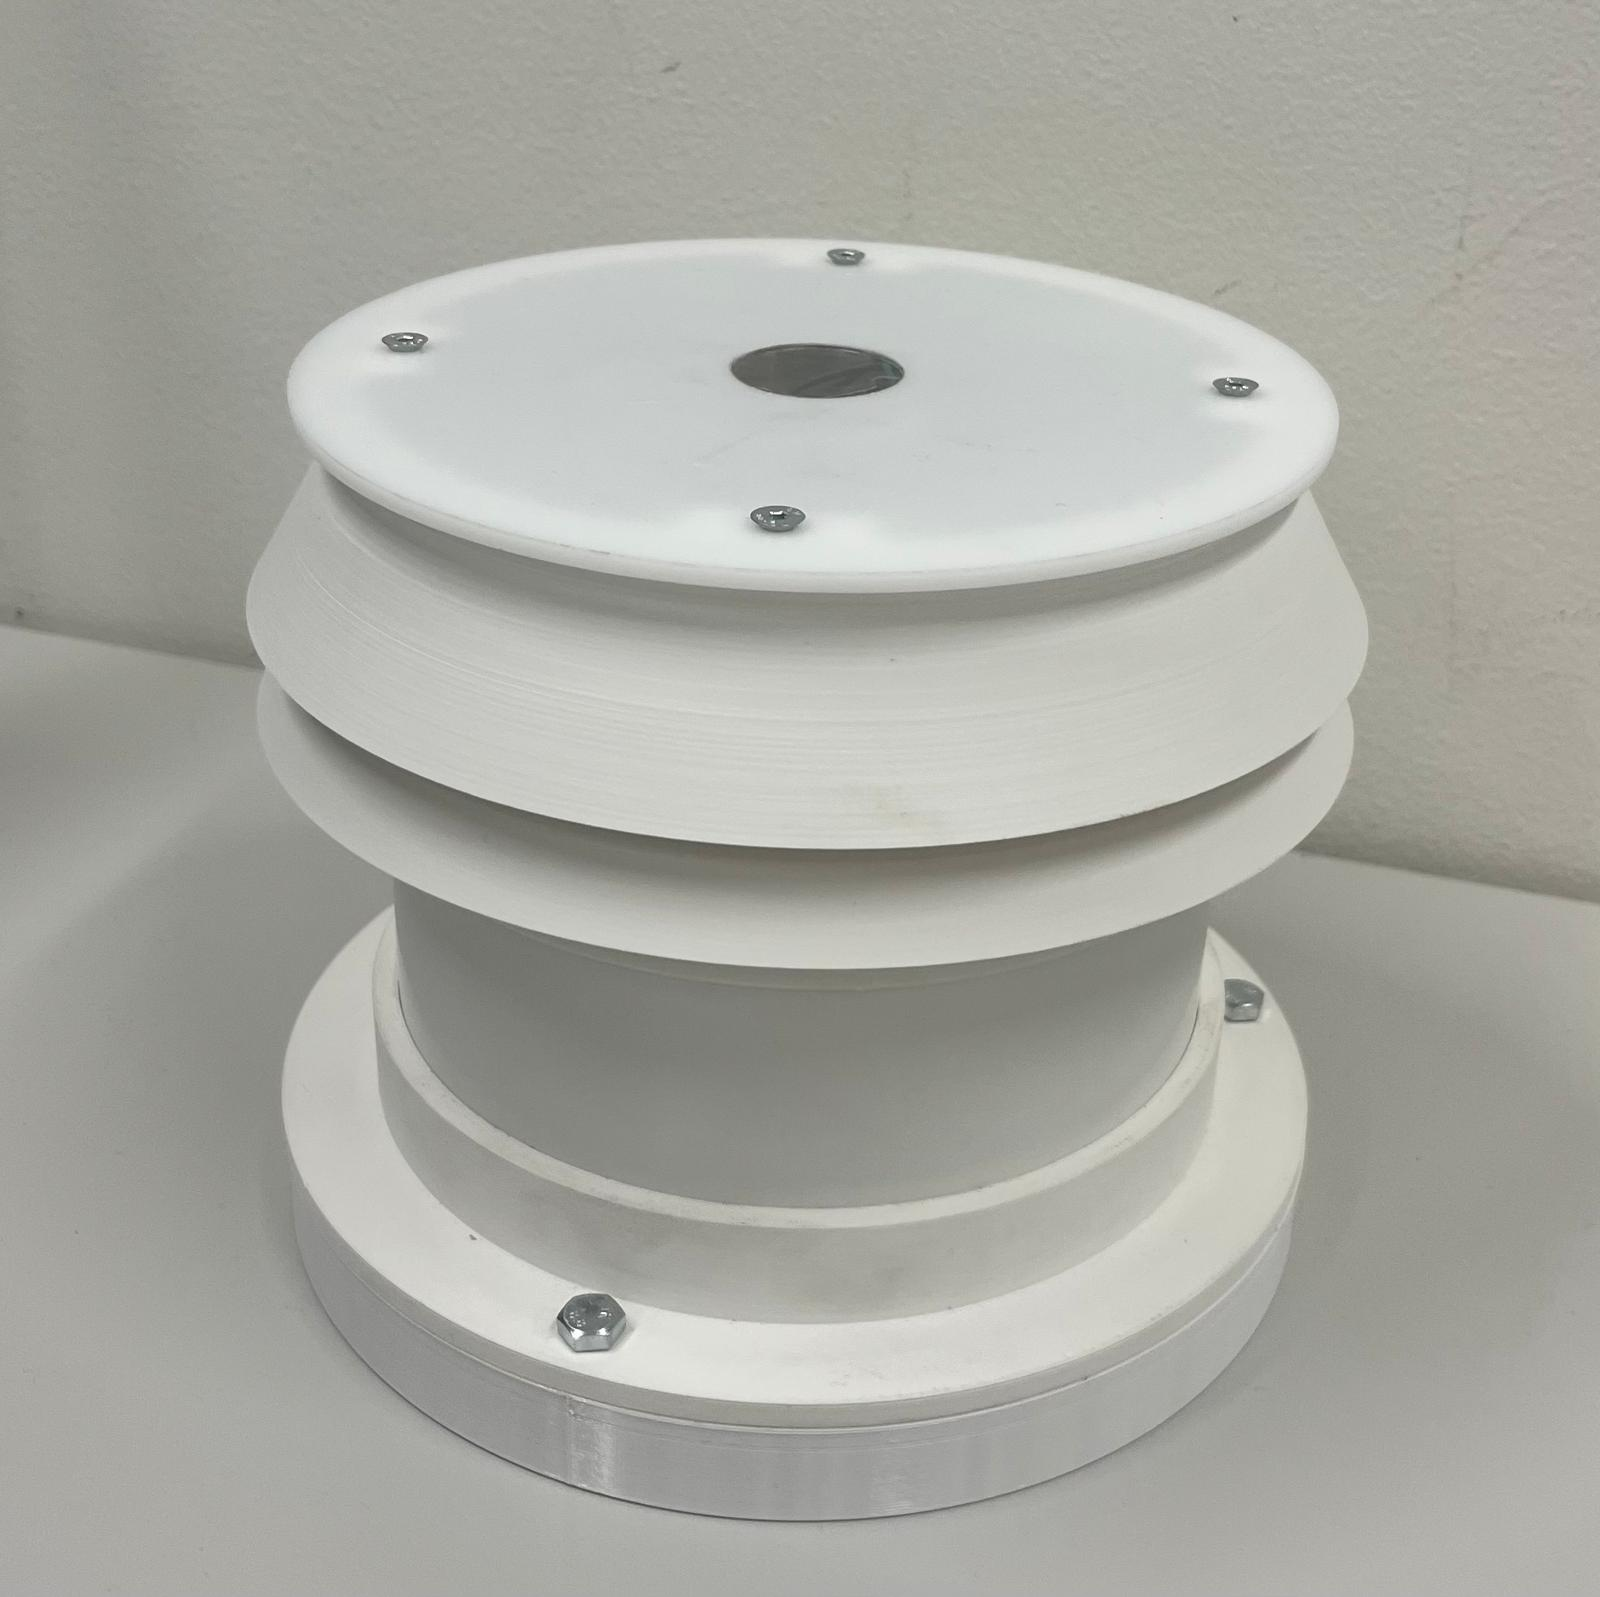
\includegraphics[width=0.4\textwidth]{images/station_full.jpeg}\par}
  \vspace{0.1cm}

  \vfill
  {\large Lausanne, Mai 2026\par}

\end{titlepage}

\thispagestyle{empty}
\clearpage
\tableofcontents
\clearpage

\section{Introduction}\label{sec:introduction}

\subsection{Contexte : le projet Sailowtech}

\begin{figure}[H]
  \centering
  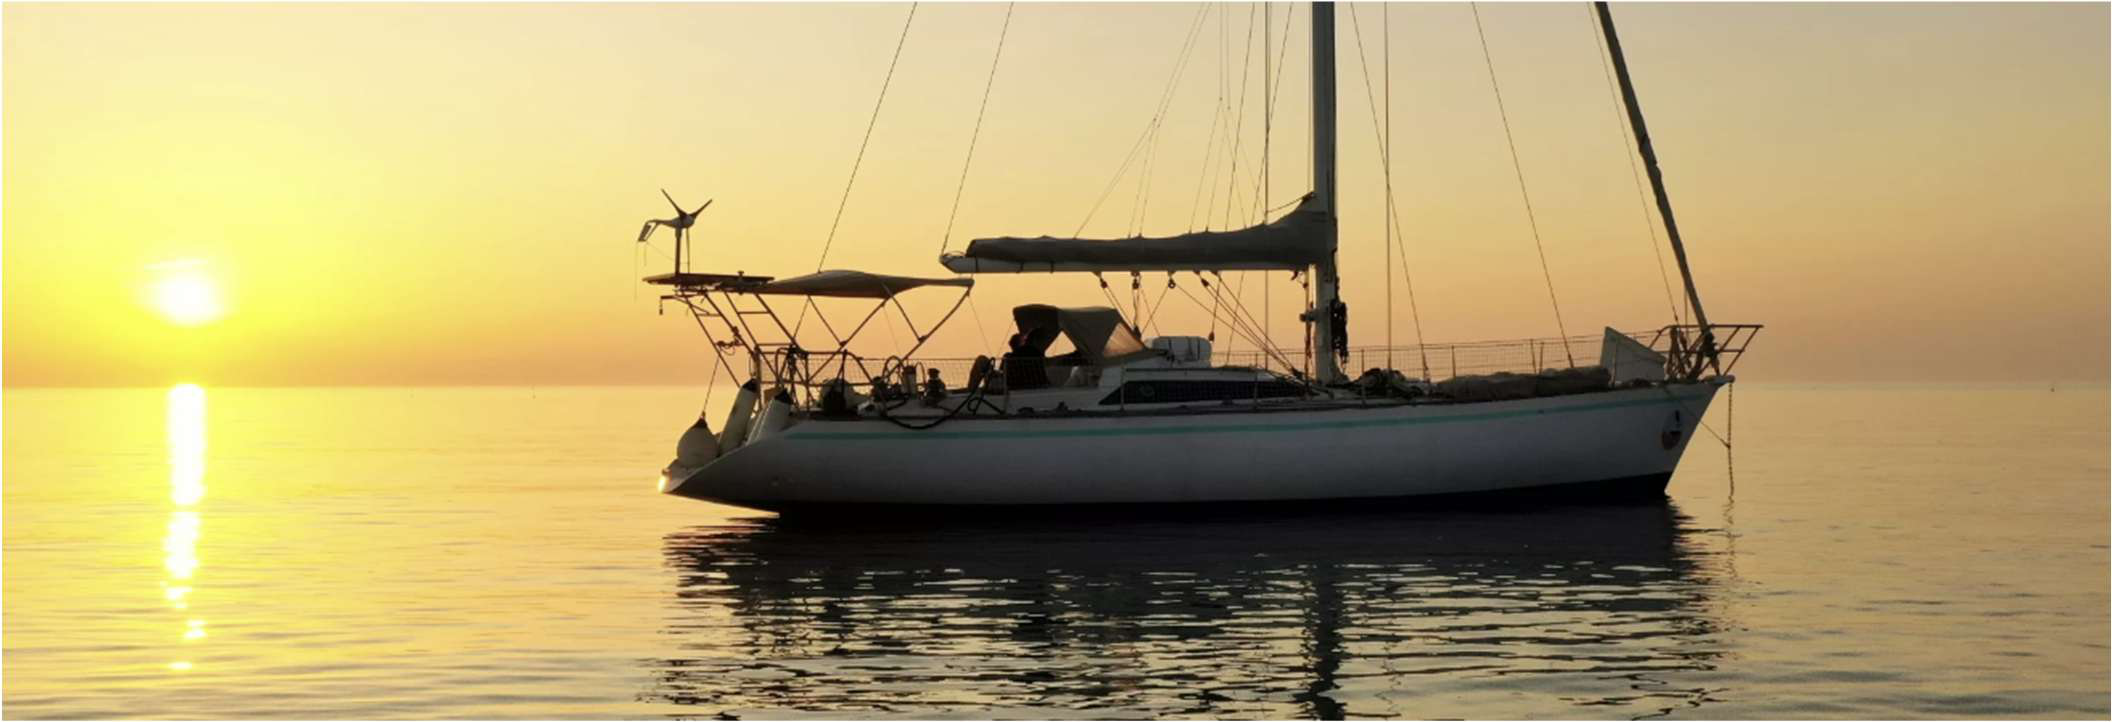
\includegraphics[width=0.7\textwidth]{images/voilier_sunset.png}
  \caption{Un voilier équipé de la station Sailowtech en expédition.}
  \label{fig:voilier}
\end{figure}

\textit{Sailowtech} est une initiative dont l'objectif est de rendre l'océanographie
plus accessible et durable en équipant les expéditions à la voile d'innovations à
bas coût. L'idée centrale est de transformer des voiliers ordinaires en plateformes
de collecte de données scientifiques, sans alourdir les équipages de technologies
complexes ou coûteuses. Les données ainsi récoltées --- qualité de l'air, paramètres
de la colonne d'eau, couverture nuageuse --- alimentent des bases de données
scientifiques ouvertes sur les océans.

\subsection{Objectifs du projet}

Notre projet de semestre ME-401, supervisé par Eric Boillat du Laboratoire de
Métallurgie Thermomécanique (LMTM) de l'EPFL, consiste à concevoir et réaliser
une station météo embarquée adaptée aux contraintes d'une expédition maritime.
La station doit remplir plusieurs fonctions :

\begin{itemize}
  \item \textbf{Acquisition de données atmosphériques} : mesure des particules
    fines (PM$_{1.0}$, PM$_{2.5}$, PM$_{10}$), de l'irradiance solaire,
    de la température, de la pression et de l'humidité.
  \item \textbf{Intégration au réseau du bateau} : réception et coordination
    des données provenant d'une sonde CTD (Conductivité, Température, Profondeur)
    sous-marine et, potentiellement, du logiciel de navigation Garmin.
  \item \textbf{Résistance aux conditions marines} : protection contre les
    projections d'eau, la corrosion saline et les vibrations.
  \item \textbf{Autonomie énergétique} : alimentation par batterie avec
    régulation DC-DC embarquée.
  \item \textbf{Vision par ordinateur (bonus)} : détection automatique de la
    couverture nuageuse par analyse d'images.
\end{itemize}

\subsection{Répartition du travail}

La réalisation du projet a été partagée entre les deux membres de l'équipe :

\begin{itemize}
  \item \textbf{Design électronique} : Guilhem Destriau (responsable principal)
    et Romain Corbel.
  \item \textbf{Design mécanique} : Romain Corbel (responsable principal)
    et Guilhem Destriau.
\end{itemize}

\section{Conception électronique}\label{sec:electronique}

\subsection{Protocole de communication}\label{subsec:protocole}

La station météo joue le rôle de concentrateur (\textit{hub}) de données entre
plusieurs systèmes hétérogènes. Le schéma de communication retenu est décrit
ci-dessous et illustré en figure~\ref{fig:protocole_comm}.

\paragraph{Réseau du bateau.} Les instruments du bateau (GPS, loch, girouette,
etc.) communiquent avec la station via le protocole \textit{NMEA 2000}, basé sur
le bus CAN (Controller Area Network). Ce standard est universellement adopté dans
le domaine maritime et permet d'interconnecter des équipements de marques
différentes sur un seul câble blindé à deux fils. Un transceiver CAN dédié assure
la conversion entre le bus et l'interface SPI de l'ESP32.

\paragraph{Sonde CTD.} La sonde CTD sous-marine est reliée à la station par câble.
Plusieurs interfaces ont été étudiées : Zigbee pour une liaison sans fil courte
portée, ou câblé en RS-485, Ethernet deux fils ou RS-232. Un port dédié est prévu
sur le PCB pour accommoder ces différentes options. Le module \textit{XIAO ESP32C6}
intégré au PCB gère la communication Zigbee.

\paragraph{Transmission vers l'ordinateur.} La station transmet les données
collectées vers un ordinateur portable à bord via Wi-Fi, permettant la
visualisation et l'enregistrement en temps réel sans liaison filaire.

\begin{figure}[H]
  \centering
  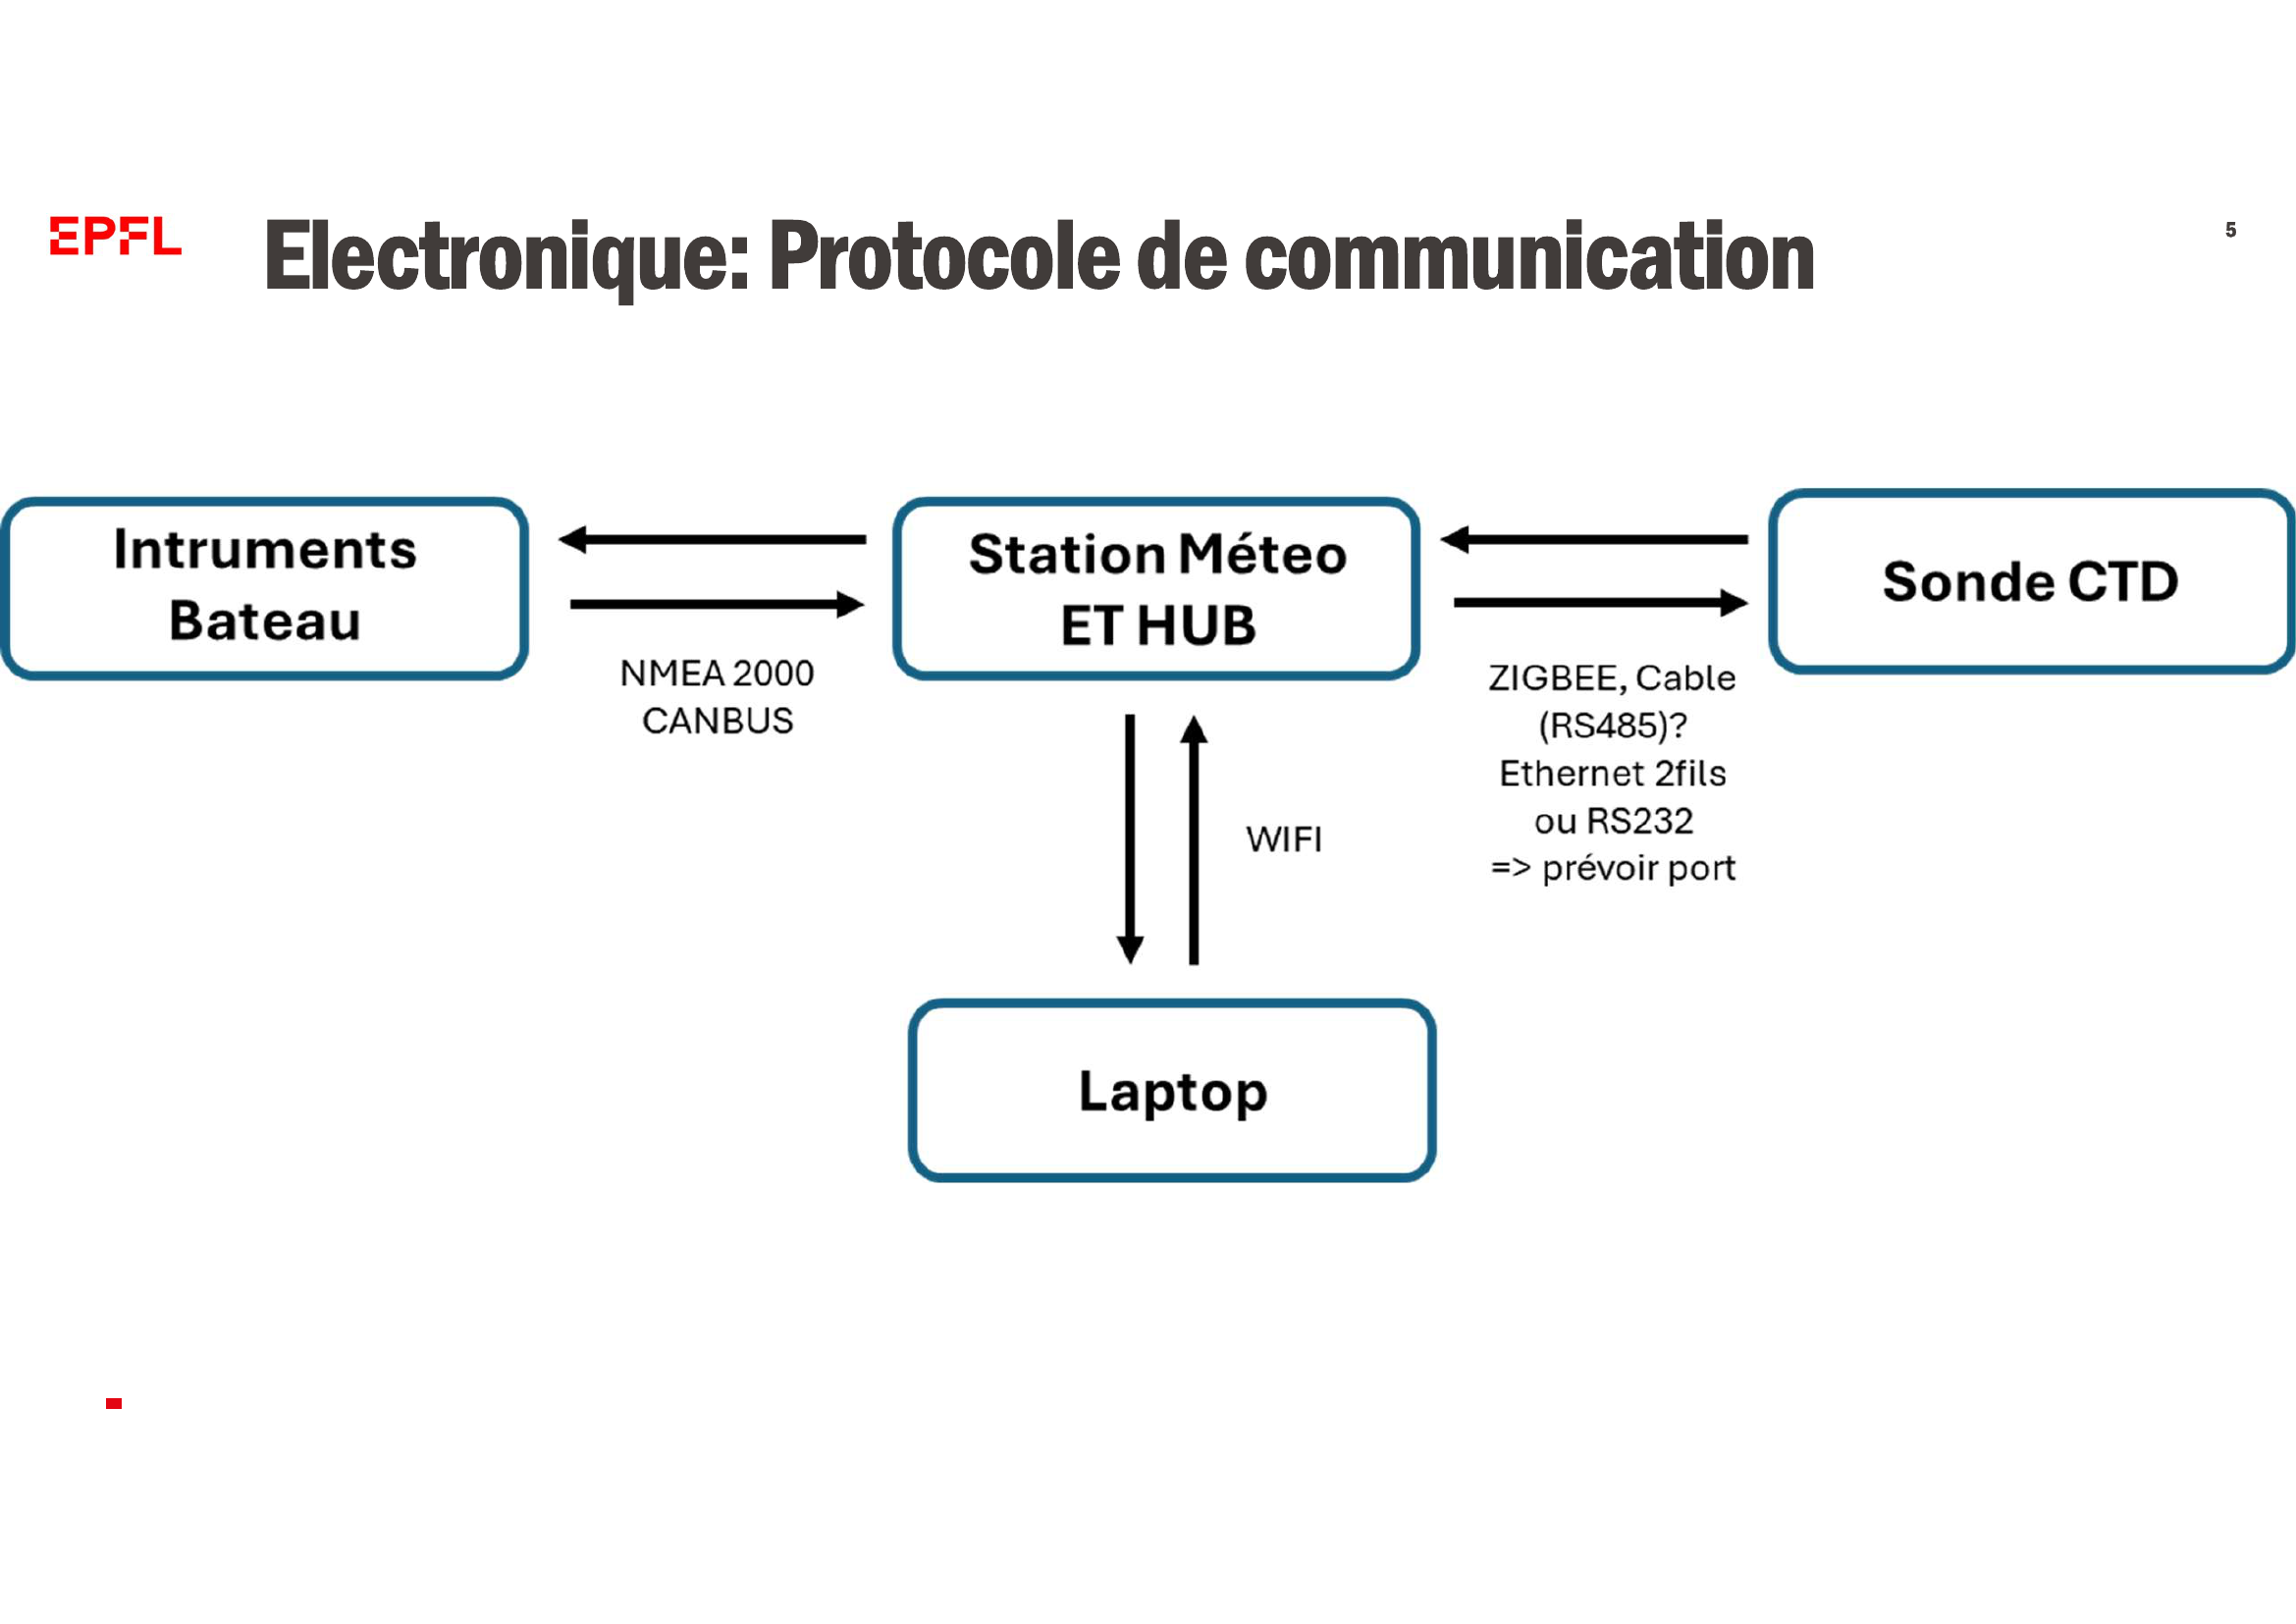
\includegraphics[width=0.85\textwidth]{images/protocole_comm.png}
  \caption{Schéma du protocole de communication entre les différents systèmes.}
  \label{fig:protocole_comm}
\end{figure}

\subsection{PCB étage 1 — Contrôle et connectivité}\label{subsec:pcb1}

Le premier étage regroupe les composants dédiés au traitement central, à la
connectivité réseau et à l'alimentation. La carte est de forme circulaire pour
s'insérer dans le boîtier cylindrique décrit à la section~\ref{sec:mecanique}.
Les composants retenus sont listés dans le tableau~\ref{tab:pcb1}.

\begin{table}[H]
  \centering
  \caption{Composants du PCB étage 1.}
  \label{tab:pcb1}
  \begin{tabular}{llc}
    \toprule
    \textbf{Fonction} & \textbf{Référence} & \textbf{Qté} \\
    \midrule
    Microcontrôleur principal & ESP32 DevKit M V1         & 1 \\
    Module Zigbee             & XIAO ESP32C6              & 1 \\
    Lecteur carte SD          & Adafruit micro SD         & 1 \\
    GPS                       & Adafruit GPS              & 1 \\
    Transceiver CAN           & MCP2515 (NMEA 2000)       & 1 \\
    Convertisseur de niveaux  & Bi-Directional Converter  & 1 \\
    Régulateur DC-DC          & Purecrea LM2596           & 1 \\
    \bottomrule
  \end{tabular}
\end{table}

\paragraph{Microcontrôleur.} L'\textit{ESP32 DevKit M V1} est choisi pour sa
double connectivité Wi-Fi et Bluetooth, sa puissance de calcul (240 MHz, deux
cœurs) et son large écosystème de bibliothèques Arduino/PlatformIO. Il orchestre
la totalité des échanges entre les capteurs, le stockage et la transmission.

\paragraph{Stockage et localisation.} La carte SD (interfacée en SPI) assure
l'enregistrement local des mesures en cas de perte de connexion Wi-Fi. Le module
GPS fournit l'horodatage et la position géographique de chaque mesure, indispensables
pour la corrélation avec d'autres sources de données oceanographiques.

\paragraph{Alimentation.} Le régulateur buck \textit{LM2596} convertit la tension
batterie (typiquement 12 V) en 5 V pour alimenter l'ensemble du système. Le
convertisseur de niveaux logiques bidirectionnel est nécessaire pour l'interfaçage
entre les composants 3,3 V (ESP32) et 5 V (certains capteurs et le transceiver CAN).

\begin{figure}[H]
  \centering
  \begin{subfigure}[b]{0.48\textwidth}
    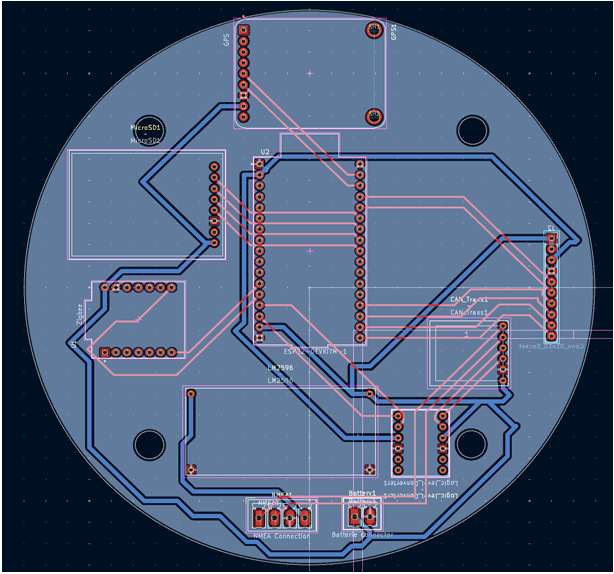
\includegraphics[width=\textwidth]{images/pcb1_routage.png}
    \caption{Routage KiCad}
  \end{subfigure}
  \hfill
  \begin{subfigure}[b]{0.48\textwidth}
    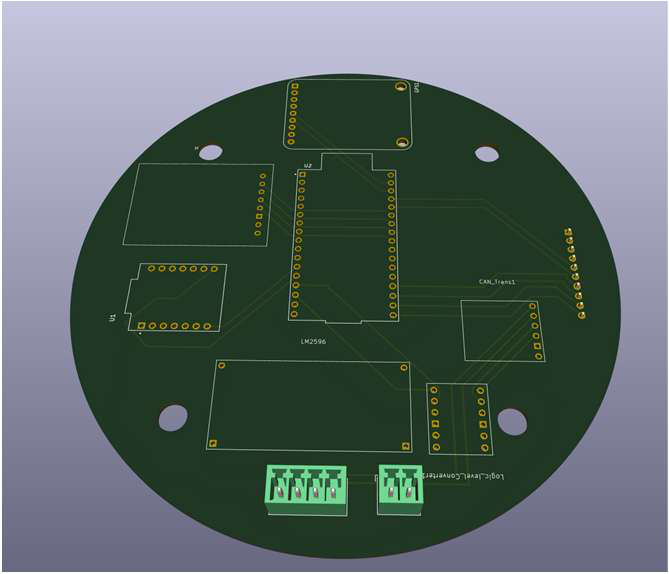
\includegraphics[width=\textwidth]{images/pcb1_3d.png}
    \caption{Rendu 3D}
  \end{subfigure}
  \caption{PCB étage 1 : contrôle et connectivité.}
  \label{fig:pcb1}
\end{figure}

\subsection{PCB étage 2 — Capteurs}\label{subsec:pcb2}

Le deuxième étage regroupe l'ensemble des capteurs environnementaux.
Les composants retenus sont listés dans le tableau~\ref{tab:pcb2}.

\begin{table}[H]
  \centering
  \caption{Composants du PCB étage 2.}
  \label{tab:pcb2}
  \begin{tabular}{llc}
    \toprule
    \textbf{Fonction}                    & \textbf{Référence}        & \textbf{Qté} \\
    \midrule
    Accéléromètre 6 axes                 & Purecrea MPU-6050         & 1 \\
    Température / Pression / Humidité    & BME280                    & 1 \\
    Capteur de lumière                   & BH1750                    & 1 \\
    Caméra                               & Joy-it ESP32 camera board & 1 \\
    Capteur de particules fines          & SPS30 (Sensirion)         & 1 \\
    \bottomrule
  \end{tabular}
\end{table}

\paragraph{Qualité de l'air.} Le capteur \textit{SPS30} de Sensirion mesure la
concentration massique des particules PM$_{1.0}$, PM$_{2.5}$, PM$_4$ et PM$_{10}$
par diffraction laser. Sa précision et sa robustesse en font un standard dans les
réseaux de surveillance de la qualité de l'air.

\paragraph{Météorologie.} Le \textit{BME280} mesure simultanément la température
($\pm 1\,^{\circ}$C), la pression atmosphérique ($\pm 1$\,hPa) et l'humidité
relative ($\pm 3$\,\%). Le \textit{BH1750} fournit une mesure de l'éclairement
lumineux en lux, utilisée comme indicateur d'irradiance solaire.

\paragraph{Orientation.} L'accéléromètre \textit{MPU-6050} (IMU 6 axes : 3 axes
accélération + 3 axes gyroscope) permet de corriger les mesures en fonction de
l'orientation et du tangage/roulis du bateau. Cette correction est essentielle
pour les mesures d'irradiance et pour la segmentation d'images nuageuses.

\paragraph{Vision.} La caméra \textit{Joy-it ESP32} orientée vers le zénith
acquiert des images périodiques du ciel pour l'algorithme de détection de
couverture nuageuse décrit à la section~\ref{sec:vision}.

\begin{figure}[H]
  \centering
  \begin{subfigure}[b]{0.48\textwidth}
    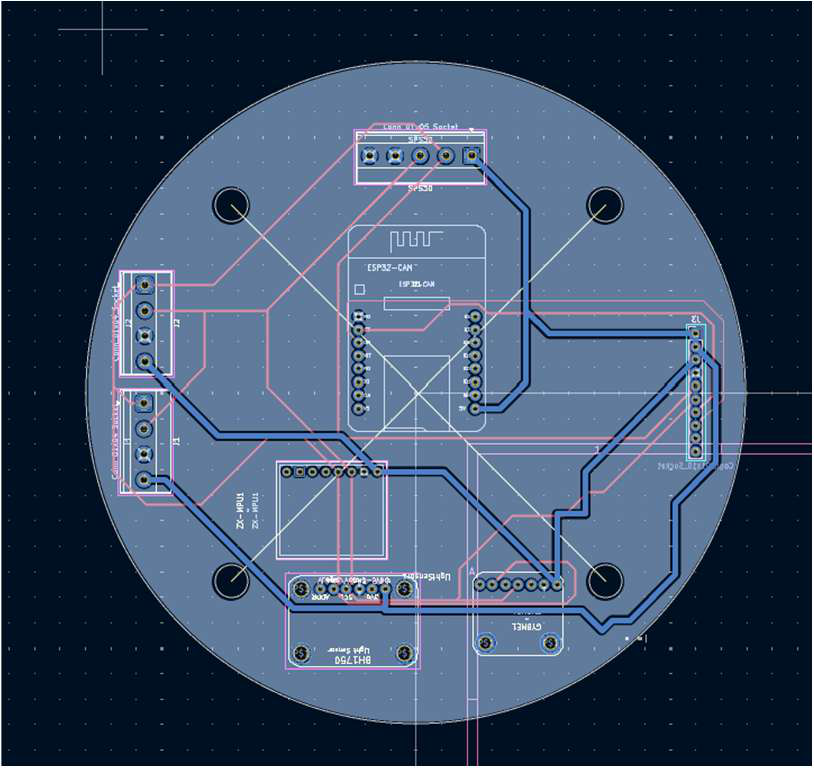
\includegraphics[width=\textwidth]{images/pcb2_routage.png}
    \caption{Routage KiCad}
  \end{subfigure}
  \hfill
  \begin{subfigure}[b]{0.48\textwidth}
    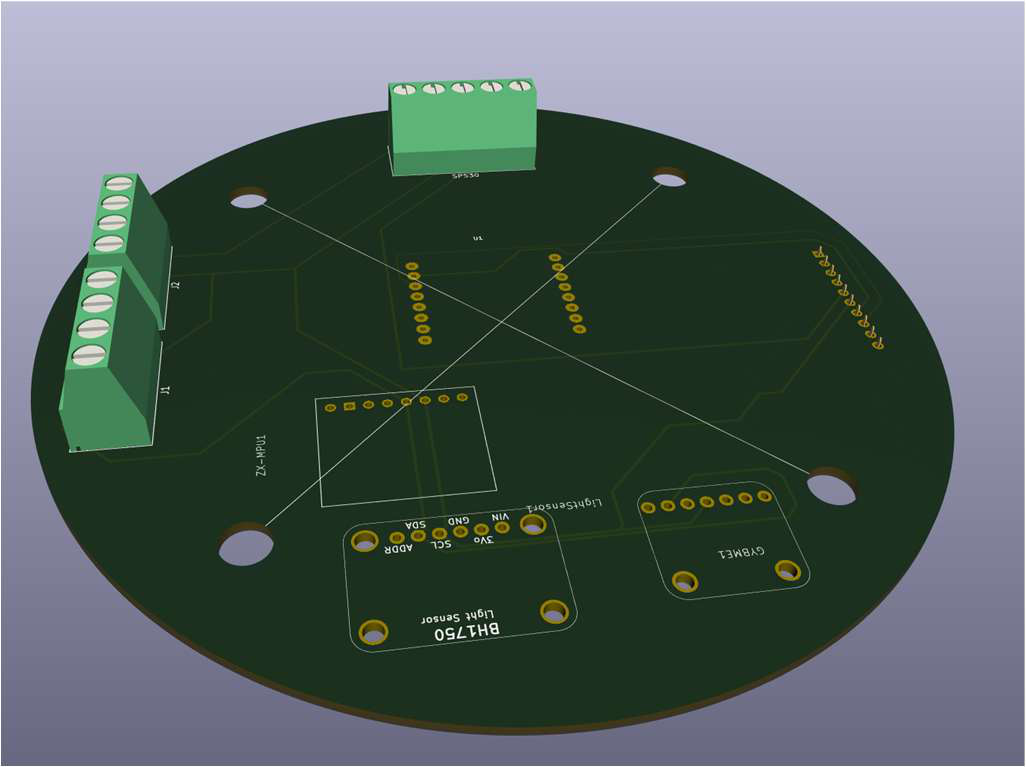
\includegraphics[width=\textwidth]{images/pcb2_3d.png}
    \caption{Rendu 3D}
  \end{subfigure}
  \caption{PCB étage 2 : capteurs environnementaux.}
  \label{fig:pcb2}
\end{figure}

\subsection{Réalisation}\label{subsec:realisation_elec}

L'ensemble des composants électroniques --- capteurs, PCB, câbles et adaptateurs
--- a été réceptionné. Les soudures et l'assemblage électronique ont été réalisés.
Un premier firmware de test a été développé pour valider la communication entre
les différents périphériques et vérifier les lectures des capteurs.

\section{Design mécanique}\label{sec:mecanique}

Le design mécanique de la station a été entièrement revu par rapport aux
concepts initiaux. L'objectif était de concevoir un boîtier à la fois
compact, résistant aux intempéries et offrant une ventilation passive
suffisante pour que les mesures de température et d'humidité ne soient
pas biaisées par l'échauffement interne.

\subsection{Structure intérieure}\label{subsec:interieur}

Les deux PCB sont empilés verticalement sur des entretoises filetées,
formant une structure en deux étages analogue à un rack miniaturisé.
Cette architecture présente plusieurs avantages :

\begin{itemize}
  \item Chaque étage est démontable indépendamment, ce qui facilite la
    maintenance et le débogage.
  \item La forme circulaire des PCB optimise l'occupation du volume
    cylindrique disponible à l'intérieur du boîtier.
  \item Les connecteurs inter-étages sont positionnés pour minimiser la
    longueur des câbles.
\end{itemize}

Des prototypes de la structure intérieure ont été réalisés par découpe
laser sur MDF, permettant de valider les cotes, les positions de fixation
et l'accessibilité aux connecteurs avant la commande des PCB définitifs
(figure~\ref{fig:interieur}).

\begin{figure}[H]
  \centering
  \begin{subfigure}[b]{0.48\textwidth}
    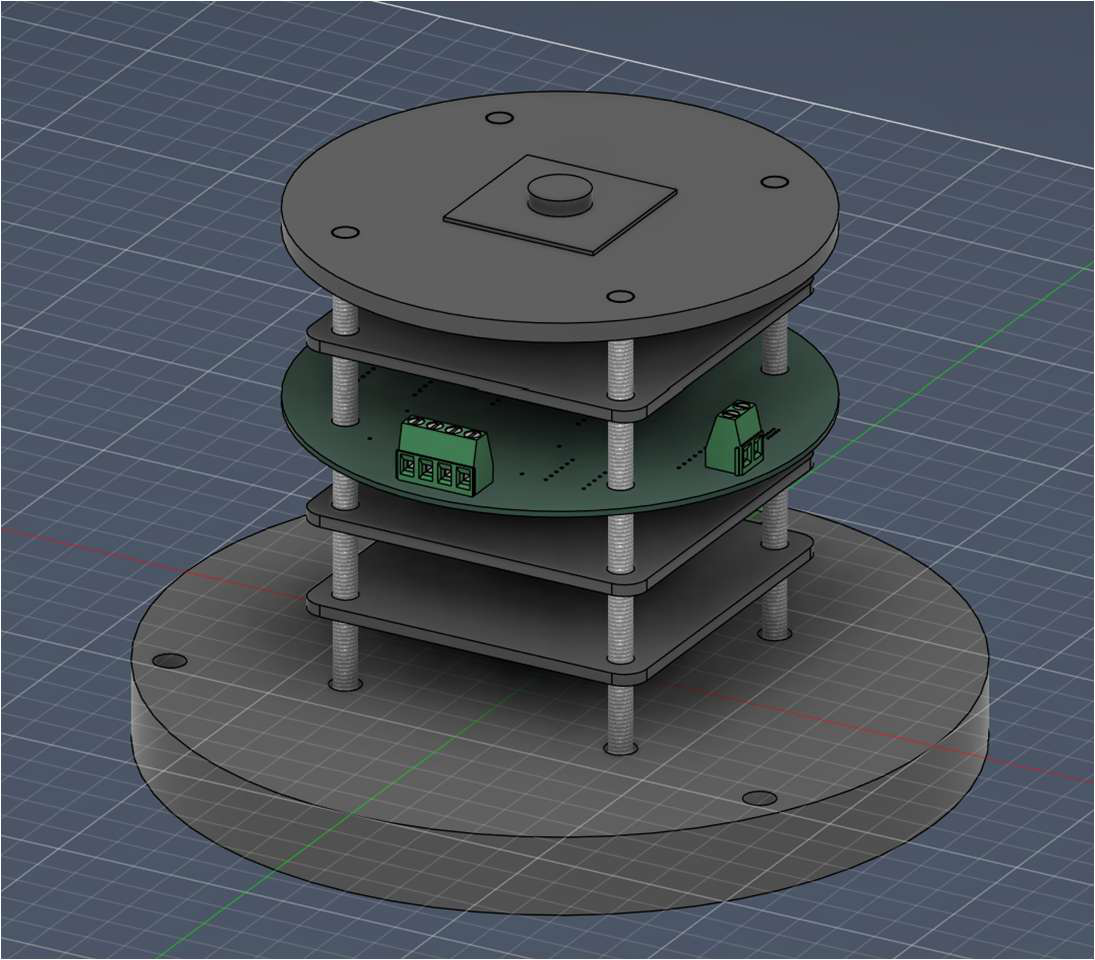
\includegraphics[width=\textwidth]{images/mecanique_interieur_cao.png}
    \caption{Rendu CAO}
  \end{subfigure}
  \hfill
  \begin{subfigure}[b]{0.48\textwidth}
    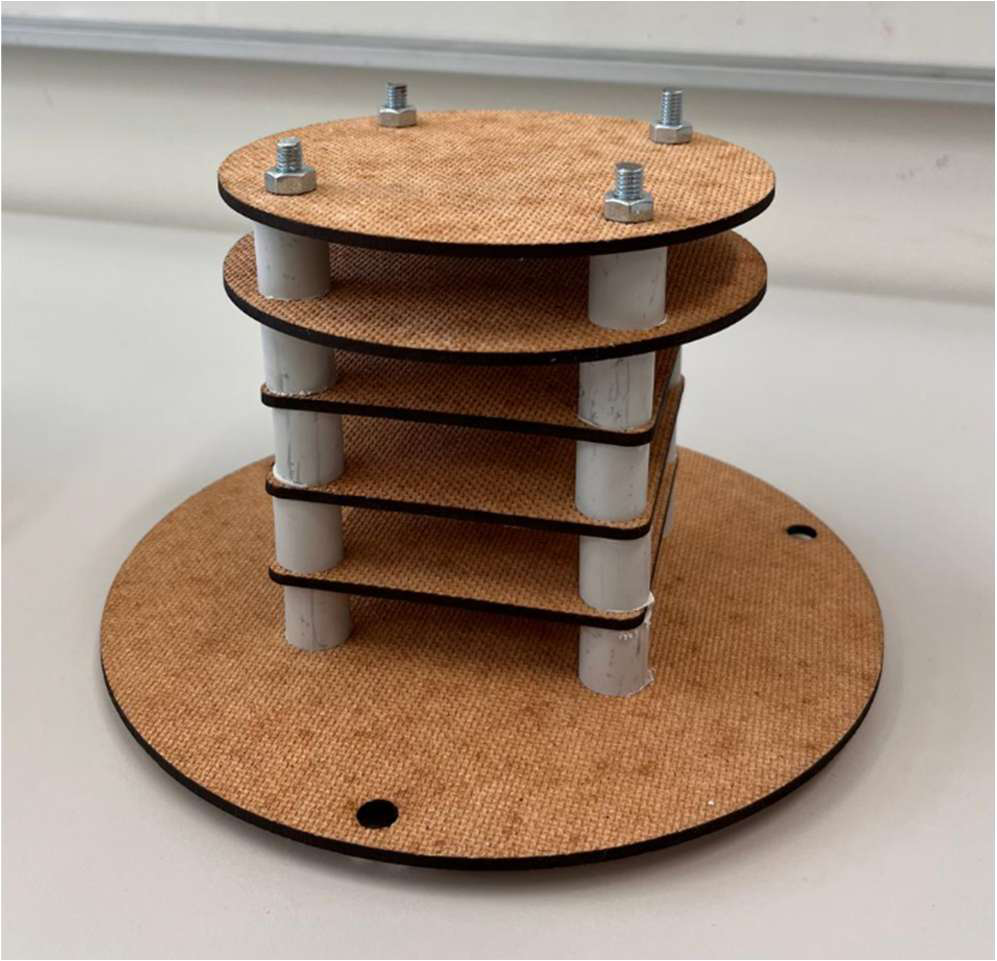
\includegraphics[width=\textwidth]{images/mecanique_interieur_photo.png}
    \caption{Prototype MDF}
  \end{subfigure}
  \caption{Structure intérieure : empilement des PCB sur entretoises.}
  \label{fig:interieur}
\end{figure}

\subsection{Boîtier extérieur}\label{subsec:exterieur}

Le boîtier extérieur s'inspire du principe de l'\textit{abri de Stevenson},
un standard météorologique historique conçu pour protéger les instruments
de mesure du rayonnement solaire direct et des précipitations, tout en
permettant la libre circulation de l'air. Notre version adapte ce concept
à une géométrie cylindrique compacte, plus adaptée à une fixation sur un
mât ou une rambarde de voilier.

La station se compose de deux parties distinctes :

\begin{itemize}
  \item \textbf{Partie basse (blanche)} : corps cylindrique en plastique blanc
    à faible absorption solaire. Des ouvertures latérales permettent la
    circulation de l'air autour des capteurs atmosphériques tout en
    bloquant les projections directes d'eau.
  \item \textbf{Chapeau supérieur (noir)} : capot orienté vers le ciel
    qui accueille la caméra sous un dôme en plexiglas transparent pour
    l'acquisition d'images nuageuses.
\end{itemize}

Des prototypes de cette enveloppe ont été réalisés en impression 3D
(PLA et PETG), permettant de valider l'assemblage et l'étanchéité des
jointures avant d'envisager des matériaux plus durables pour une
utilisation marine prolongée. Des membranes \textit{Gore-Tex} ont
également été intégrées dans les tests pour évaluer leur capacité à
assurer la ventilation tout en empêchant les entrées d'eau.

\begin{figure}[H]
  \centering
  \begin{subfigure}[b]{0.48\textwidth}
    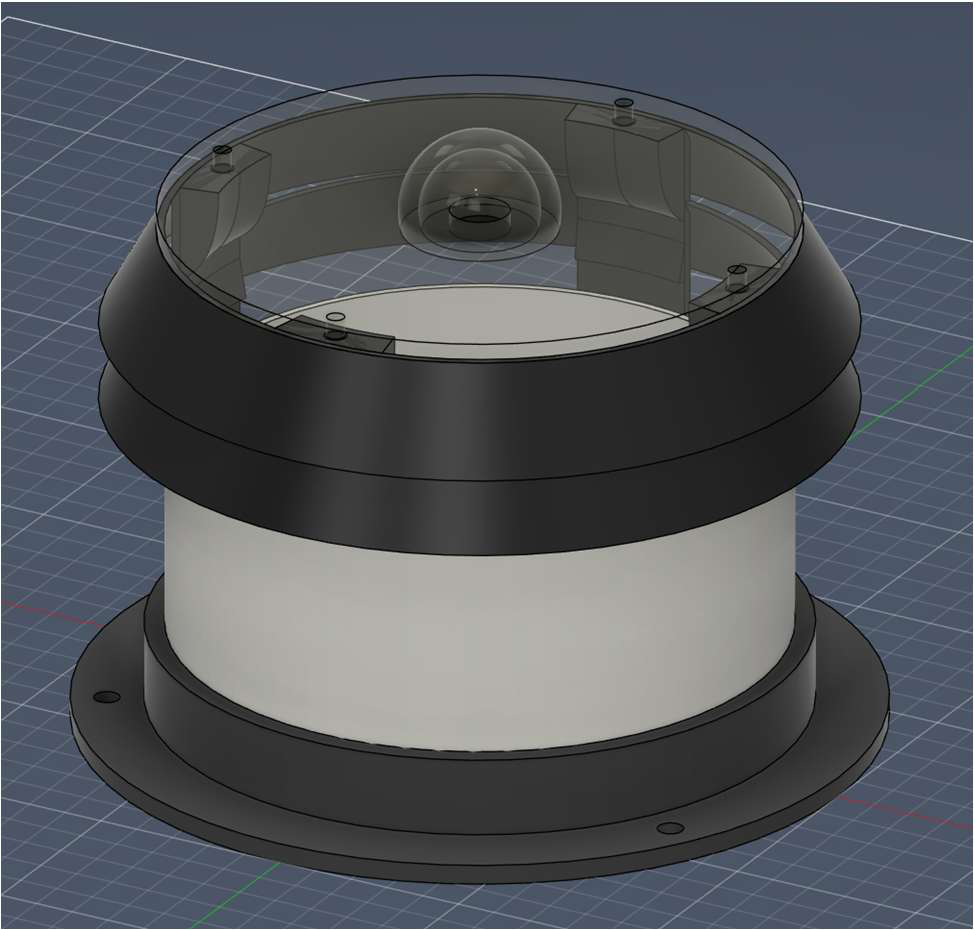
\includegraphics[width=\textwidth]{images/mecanique_boitier_cao.png}
    \caption{Rendu CAO}
  \end{subfigure}
  \hfill
  \begin{subfigure}[b]{0.48\textwidth}
    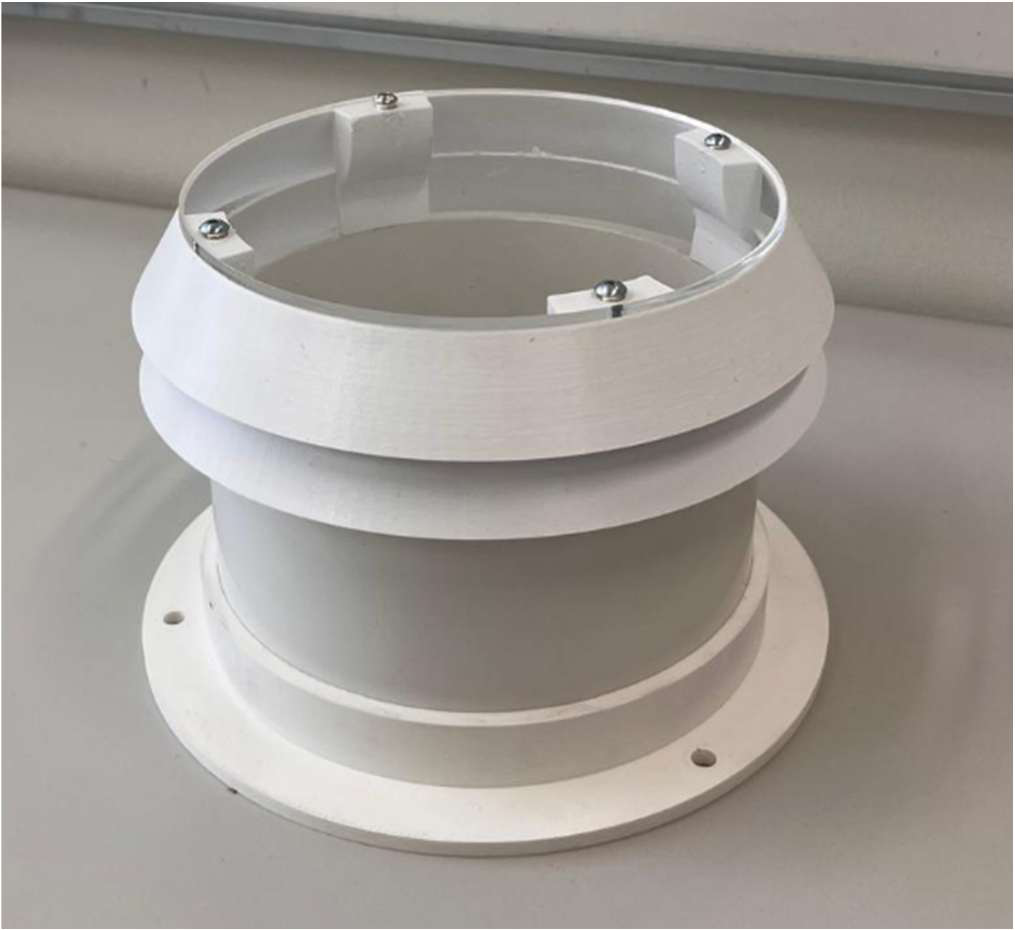
\includegraphics[width=\textwidth]{images/mecanique_boitier_photo.png}
    \caption{Prototype imprimé 3D}
  \end{subfigure}
  \caption{Boîtier extérieur : chapeau noir (caméra) et corps blanc (ventilation).}
  \label{fig:exterieur}
\end{figure}

\begin{figure}[H]
  \centering
  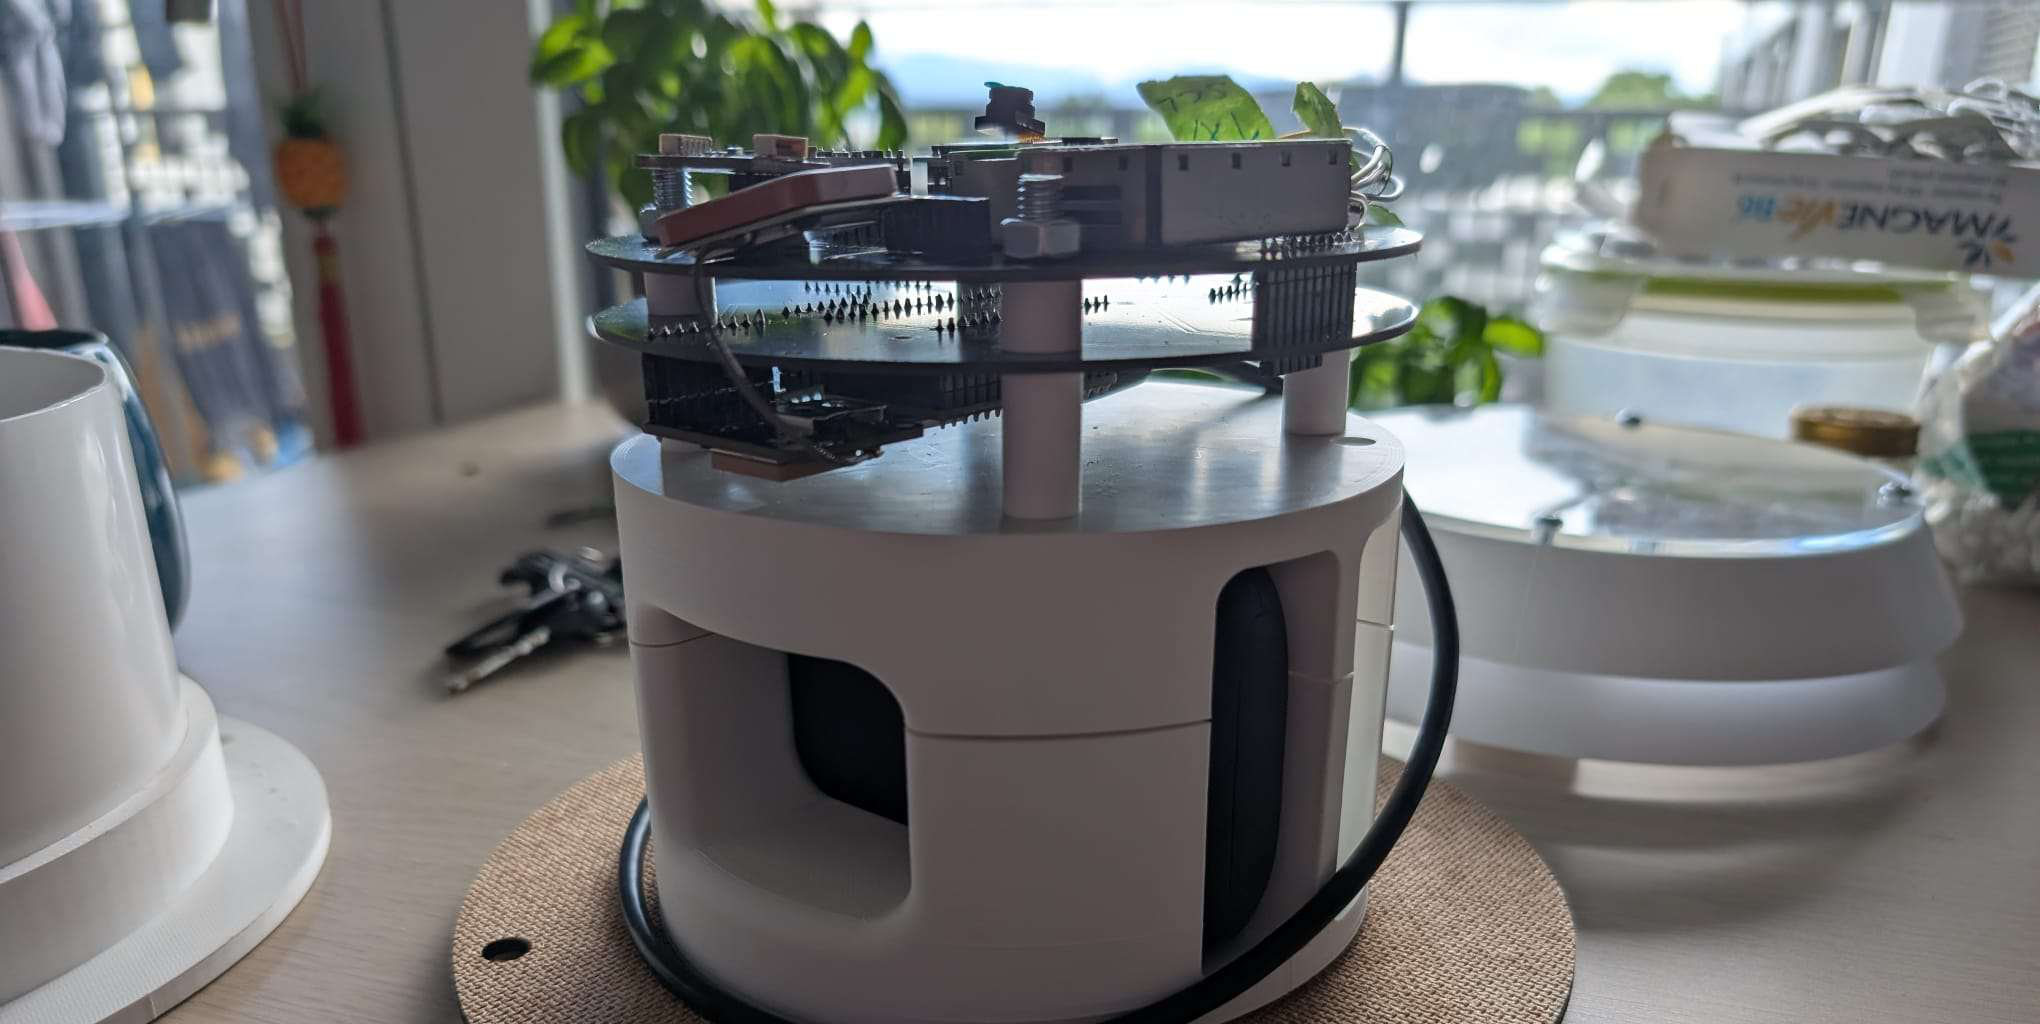
\includegraphics[width=0.5\textwidth]{images/station_assemblée.png}
  \caption{Station assemblée avec les PCBs montés sur la structure intérieure.}
  \label{fig:station_assemblée}
\end{figure}

\subsection{Problèmes identifiés et solutions}\label{subsec:problemes_meca}

Deux risques ont été identifiés lors des tests préliminaires et font
l'objet d'investigations spécifiques.

\paragraph{Effet de serre lié au dôme en plexiglas.}
Le plexiglas est transparent au rayonnement visible mais partiellement
opaque au rayonnement infrarouge thermique. Il pourrait donc créer un
effet de serre local sous le capot supérieur, biaisant les mesures de
température et d'humidité si les capteurs se trouvent à proximité. Des
mesures comparatives sont prévues pour quantifier cet écart. Si l'effet
est significatif, la plaque supérieure sera remplacée par un matériau
ajouré ou traité antireflet, ou les capteurs sensibles seront déplacés
vers la partie basse du boîtier.

\paragraph{Ventilation suffisante.}
L'abri de Stevenson repose sur la convection naturelle. Sur un voilier
en mouvement, le vent relatif est généralement suffisant pour assurer
un renouvellement d'air permanent. Pour les situations de calme plat,
une alternative basée sur un tube en coude (aspiration passive par
effet venturi du vent résiduel) a été envisagée. Cette solution
nécessiterait toutefois l'ajout d'un ventilateur en l'absence de vent,
ce qui augmente la complexité et la consommation électrique. Les tests
en conditions réelles permettront de trancher.

\begin{figure}[H]
  \centering
  \begin{subfigure}[b]{0.35\textwidth}
    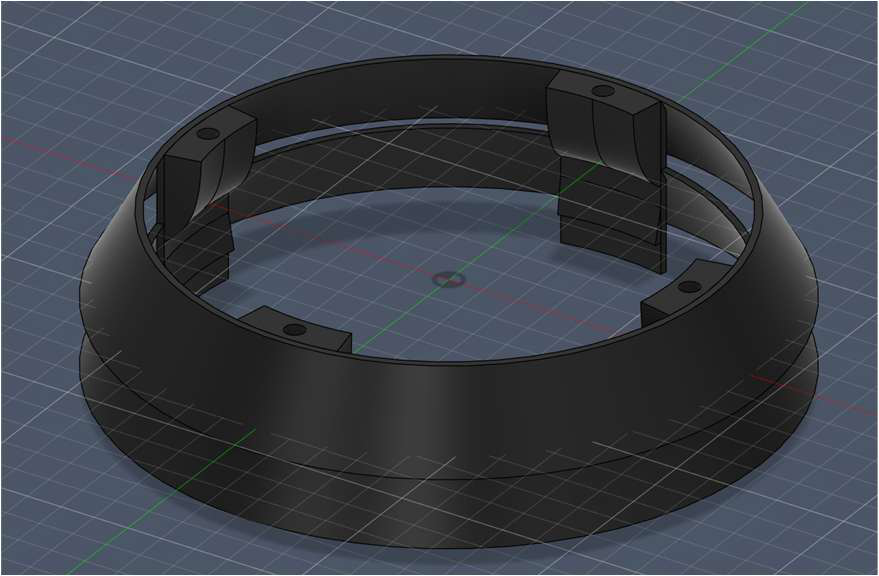
\includegraphics[width=\textwidth]{images/mecanique_stevenson_anneau.png}
    \caption{Anneau de ventilation (CAO)}
  \end{subfigure}
  \hfill
  \begin{subfigure}[b]{0.55\textwidth}
    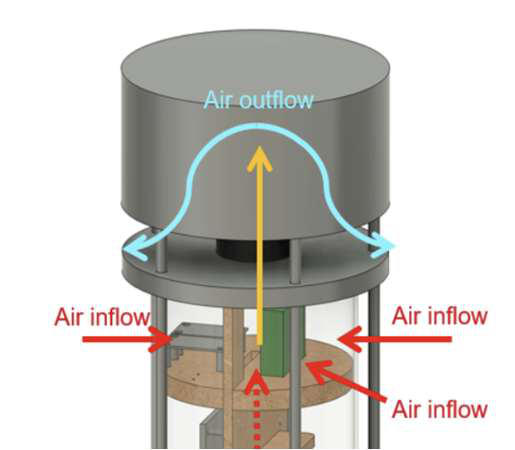
\includegraphics[width=\textwidth]{images/mecanique_ventilation.png}
    \caption{Schéma de circulation d'air}
  \end{subfigure}
  \caption{Ventilation passive : entrées d'air latérales et sortie par le haut.}
  \label{fig:ventilation}
\end{figure}

\section{Vision par ordinateur}\label{sec:vision}

\subsection{Objectif}

La couverture nuageuse est une variable clé pour la caractérisation du
rayonnement solaire reçu par la surface de la mer. Les capteurs commerciaux
de nébulosité (pyranomètres, détecteurs infrarouge) sont coûteux et peu adaptés
à une intégration compacte dans une station embarquée. Une approche par vision
par ordinateur a donc été explorée comme alternative bas coût, en s'appuyant
sur la caméra déjà présente sur le PCB étage 2.

\subsection{Méthode : segmentation par seuillage HSV}

La caméra \textit{Joy-it ESP32} est orientée vers le zénith sous le dôme en
plexiglas. Elle capture des images périodiques du ciel. L'algorithme de
traitement repose sur une segmentation en deux étapes :

\begin{enumerate}
  \item \textbf{Conversion HSV.} L'image RGB est convertie dans l'espace
    colorimétrique HSV (Teinte, Saturation, Valeur). Cet espace sépare
    l'information de couleur (teinte) de la luminosité (valeur) et de la
    pureté de la couleur (saturation), ce qui le rend plus robuste aux
    variations d'exposition que le RVB direct.

  \item \textbf{Seuillage.} Les nuages, plus blancs et moins saturés que le
    ciel bleu, sont isolés par un masque combinant une saturation basse et
    une valeur élevée. Le seuil est déterminé empiriquement sur un ensemble
    d'images représentatives de différentes conditions météorologiques.
\end{enumerate}

Le taux de couverture nuageuse est calculé comme le rapport entre le nombre
de pixels classés ``nuage'' et le nombre total de pixels de l'image, après
exclusion des bords occupés par le boîtier.

\begin{figure}[H]
  \centering
  \begin{subfigure}[b]{0.48\textwidth}
    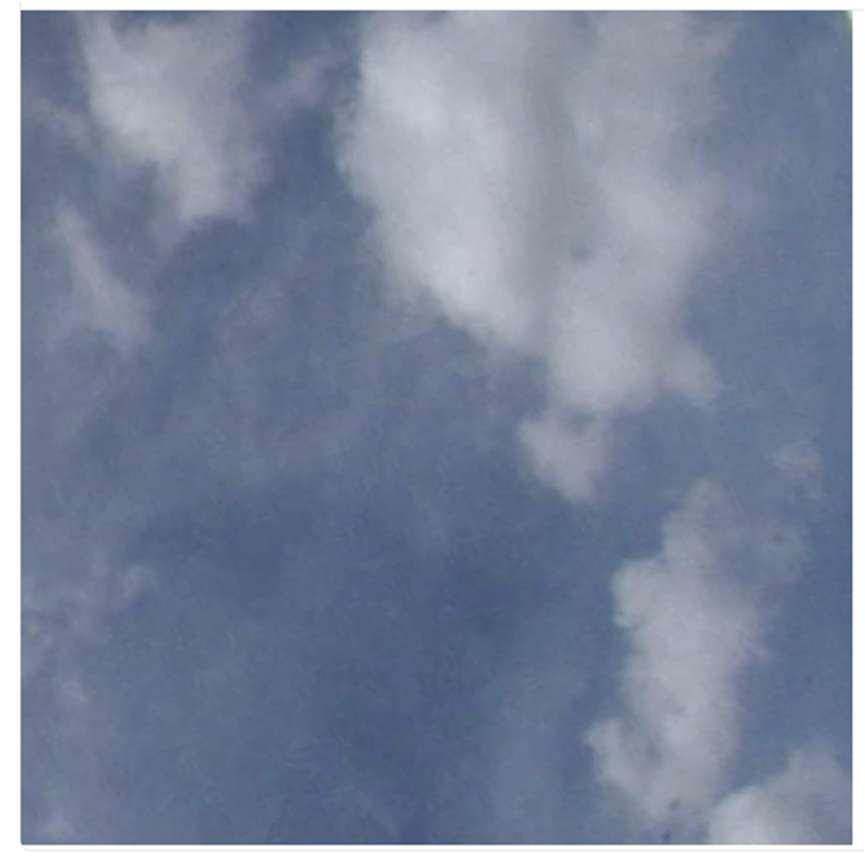
\includegraphics[width=\textwidth]{images/vision_ciel.png}
    \caption{Image brute du ciel}
  \end{subfigure}
  \hfill
  \begin{subfigure}[b]{0.48\textwidth}
    
\includegraphics[width=\textwidth]{images/vision_masque.png}
    \caption{Masque binaire (blanc = nuage)}
  \end{subfigure}
  \caption{Exemple de segmentation nuages/ciel par seuillage HSV.}
  \label{fig:cv_segmentation}
\end{figure}

\subsection{Résultats et perspectives}

Les tests préliminaires montrent que l'algorithme discrimine correctement
les nuages blancs sur fond de ciel bleu dans des conditions standard
(figure~\ref{fig:cv_segmentation}). Plusieurs cas difficiles restent à traiter :

\begin{itemize}
  \item \textbf{Ciel uniformément couvert} : sans contraste bleu/blanc,
    le seuillage par saturation devient peu fiable.
  \item \textbf{Coucher et lever de soleil} : la teinte du ciel vire
    vers l'orange/rouge, perturbant le masque basé sur la teinte bleue.
  \item \textbf{Éblouissement direct} : lorsque le soleil entre dans
    le champ de la caméra, la surexposition locale crée de faux positifs.
\end{itemize}

Pour améliorer la robustesse, deux pistes sont envisagées : l'adaptation
dynamique du seuil en fonction de l'heure et de la position GPS (azimut
solaire calculé), et l'entraînement d'un classifieur léger (réseau de
neurones convolutionnel de petite taille ou k-means sur l'histogramme HSV)
utilisable sur le microcontrôleur ESP32 ou sur l'ordinateur de bord.

\section{Conclusion et perspectives}\label{sec:conclusion}

Ce projet de semestre ME-401 a permis de concevoir et de réaliser les
premières versions fonctionnelles d'une station météo embarquée pour les
expéditions à la voile dans le cadre du projet Sailowtech.

\subsection{Bilan des travaux}

Les travaux accomplis couvrent l'ensemble de la chaîne, de la conception
jusqu'à la validation préliminaire :

\begin{itemize}
  \item \textbf{Architecture électronique} : conception et routage de deux
    PCB circulaires (étage contrôle et étage capteurs), réception de
    l'ensemble des composants, soudure et assemblage réalisés.

  \item \textbf{Firmware} : développement d'un premier firmware de
    validation (lecture des capteurs, enregistrement SD, communication
    Wi-Fi) et d'un module de vision par ordinateur pour la détection
    de la couverture nuageuse.

  \item \textbf{Design mécanique} : conception d'un boîtier cylindrique
    inspiré de l'abri de Stevenson, réalisation de prototypes par
    impression 3D et découpe laser, intégration de membranes Gore-Tex
    pour tester la ventilation étanche.
\end{itemize}

\subsection{Travaux restants}

Les prochaines étapes pour finaliser et valider la station sont :

\begin{enumerate}
  \item Tester la résistance mécanique du boîtier et son étanchéité
    en conditions simulées (aspersions d'eau, chocs).
  \item Quantifier l'effet de serre du dôme en plexiglas et adapter
    le design si nécessaire.
  \item Évaluer la ventilation passive dans différentes conditions de vent
    et valider que les mesures de température ne sont pas biaisées.
  \item Intégrer et valider l'ensemble de la chaîne de mesure lors d'une
    sortie en mer avec l'équipe Sailowtech.
  \item Améliorer l'algorithme de vision par ordinateur pour les cas
    difficiles (ciel couvert uniforme, contre-jour).
\end{enumerate}

\subsection{Conclusion}

La station conçue répond aux objectifs initiaux : elle est compacte,
modulaire, capable de mesurer la qualité de l'air et les paramètres
météorologiques, et peut communiquer avec les instruments du bateau via
NMEA 2000. L'intégration dans l'écosystème Sailowtech ouvre la voie à
un réseau distribué de voiliers collectant des données environnementales
en haute mer, avec un coût matériel très inférieur aux solutions
professionnelles existantes.


\clearpage
\bibliographystyle{unsrt}
\bibliography{references}

\end{document}
